\section{Wyniki końcowej ewaluacji}
\label{sec:wyniki-koncowej-ewaluacji}

Najpierw porównałem końcowe wyniki wszystkich ośmiu
podstawowych konfiguracji po 50\,000 epizodów treningowych.
Dla każdej konfiguracji obliczyłem średnią wartość EV z pięciu
niezależnych przebiegów treningowych oraz odchylenie standardowe między
seedami. Wyniki przedstawiam w tabeli~\ref{tab:final-ev-50k}.

\begin{table}[htbp]
    \centering
    \caption{Wyniki końcowej ewaluacji modeli po 50\,000 epizodów treningowych}
    \label{tab:final-ev-50k}
    \begin{tabular}{lllrr}
        \toprule
        Algorytm & Reprezentacja & Nagroda & Średnie EV & SD seedów \\
        \midrule
        DQN & RAW & zysk netto
            & -0{,}6450 & 0{,}0184 \\
        DQN & RAW & skalowana
            & -0{,}5681 & 0{,}0401 \\
        \textbf{DQN} & \textbf{FEATURES} & \textbf{zysk netto}
            & \textbf{-0{,}4076} & \textbf{0{,}0080} \\
        DQN & FEATURES & skalowana
            & -0{,}4165 & 0{,}0169 \\
        \midrule
        REINFORCE & RAW & zysk netto
            & -0{,}3785 & 0{,}0074 \\
        REINFORCE & RAW & skalowana
            & -0{,}3804 & 0{,}0014 \\
        REINFORCE & FEATURES & zysk netto
            & -0{,}3823 & 0{,}0014 \\
        \textbf{REINFORCE} & \textbf{FEATURES} & \textbf{skalowana}
            & \textbf{-0{,}3211} & \textbf{0{,}0657} \\
        \bottomrule
    \end{tabular}
\end{table}

Najwyższe średnie EV spośród wariantów DQN uzyskała konfiguracja
FEATURES z funkcją nagrody opartą na zysku netto. Jej średni wynik
wyniósł $-0{,}4076$. Dla REINFORCE najwyższy średni wynik uzyskała
konfiguracja FEATURES ze skalowaną funkcją nagrody, dla której średnie
EV wyniosło $-0{,}3211$.

Widoczna jest wyraźna różnica w zmienności tych wyników.
Dla wspomnianego wariantu DQN odchylenie standardowe między pięcioma
seedami wyniosło jedynie $0{,}0080$, natomiast dla konfiguracji
REINFORCE FEATURES ze skalowaną nagrodą osiągnęło $0{,}0657$.
Oznacza to, że wysoka średnia wartość EV wariantu REINFORCE była
związana z dużo większym zróżnicowaniem jakości polityk uzyskanych
w poszczególnych przebiegach. Do tego zjawiska wracam w dalszej części rozdziału.

Na tym samym harmonogramie 100\,000 rozdań ponownie oceniłem dwóch
agentów bazowych, Random i RuleBased. Ich wyniki przedstawiam
w tabeli~\ref{tab:baseline-ev-50k}.

\begin{table}[htbp]
    \centering
    \caption{Wyniki końcowej ewaluacji agentów bazowych}
    \label{tab:baseline-ev-50k}
    \begin{tabular}{lr}
        \toprule
        Agent & Średnie EV \\
        \midrule
        Random & -0{,}5173 \\
        RuleBased & -0{,}0106 \\
        \bottomrule
    \end{tabular}
\end{table}

Wartość uzyskana przez agenta regułowego była znacznie bliżej zera niż
wyniki wszystkich wytrenowanych modeli uczenia przez wzmacnianie.

Niemniej jednak większość konfiguracji RL osiągnęła wyższe średnie EV niż
agent losowy. Wyjątek stanowiły dwa warianty DQN wykorzystujące
reprezentację RAW, których średnie EV wyniosły odpowiednio
$-0{,}6450$ i $-0{,}5681$. Po zastosowaniu reprezentacji FEATURES
oba warianty DQN uzyskały już wynik wyższy niż agent losowy.
W przypadku REINFORCE wszystkie cztery badane konfiguracje osiągnęły
wyższe średnie EV od agenta losowego.

Zestawienie wyników poszczególnych seedów, ich średnich oraz położenia
agentów bazowych przedstawiam na rysunku~\ref{fig:final-ev-50k}. Na osi
poziomej znajduje się wartość EV, a na osi pionowej osiem konfiguracji algorytmów. 
Małe punkty przedstawiają
wyniki poszczególnych seedów, większe znaczniki średnie wartości
konfiguracji wraz z 95-procentowymi przedziałami ufności, a linie
pionowe oznaczają wyniki agentów Random i RuleBased. Widać na nim, że
rozrzut punktów wokół średniej jest podobny dla większości
konfiguracji obu algorytmów, z wyjątkiem konfiguracji REINFORCE
FEATURES ze skalowaną nagrodą, dla której jest on zauważalnie większy
niż dla pozostałych siedmiu konfiguracji, co świadczy o różnicy
w powtarzalności obu algorytmów, którą analizuję w dalszej części
rozdziału.

\begin{figure}[htbp]
    \centering
    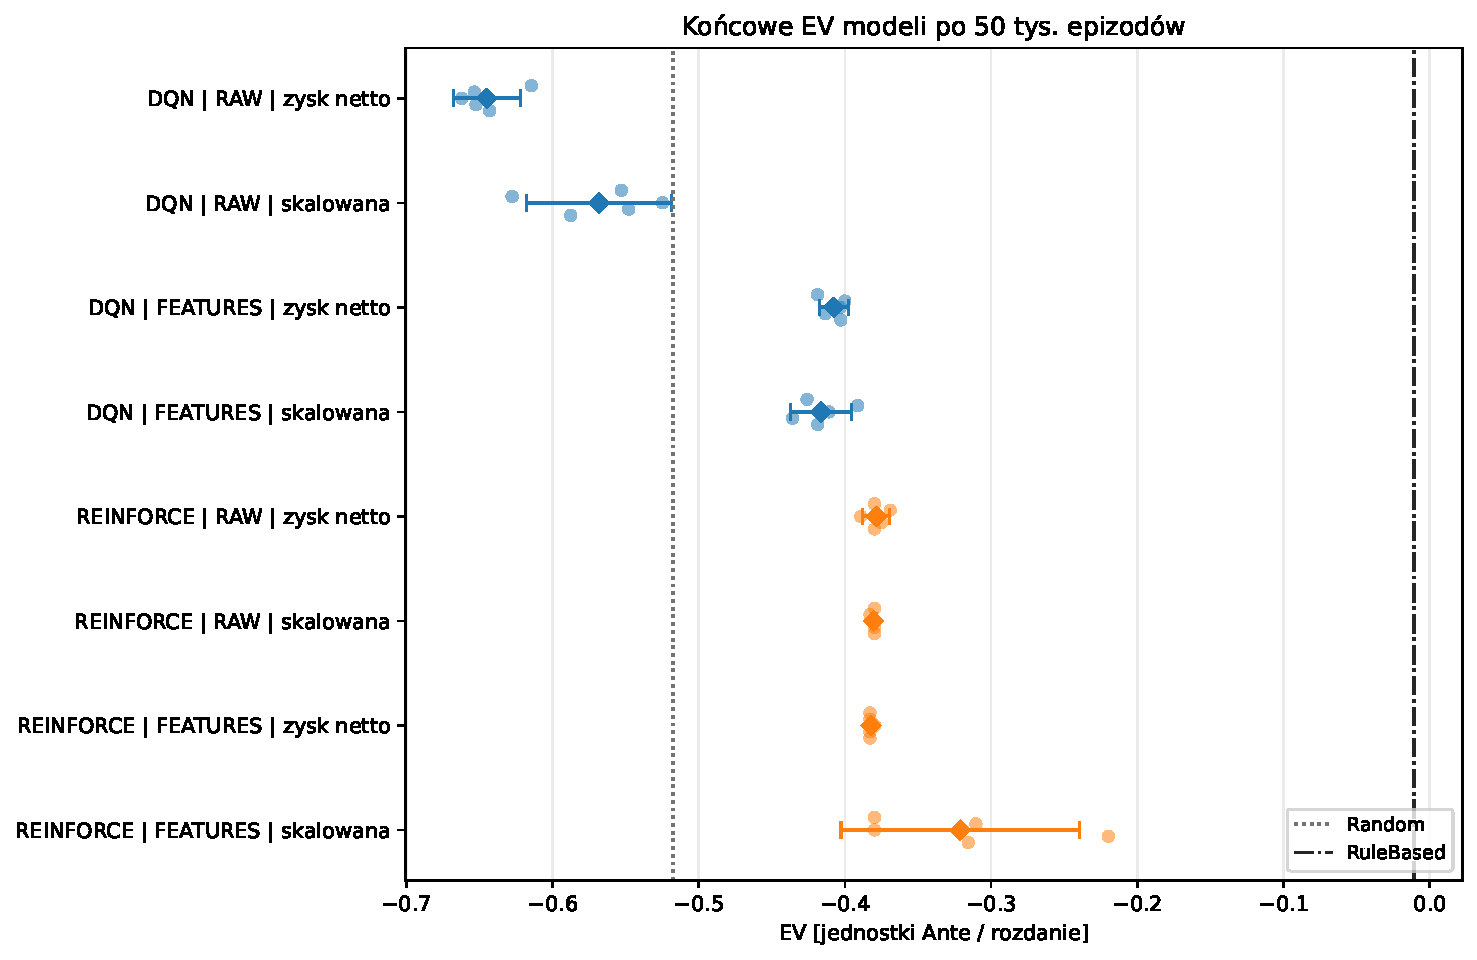
\includegraphics[
        width=\textwidth
    ]{../experiments/results/final_analysis/01_final_ev_50k.pdf}
    \caption{Końcowe EV ośmiu konfiguracji po 50\,000 epizodów
    treningowych.}
    \label{fig:final-ev-50k}
\end{figure}

Sama informacja o zastosowanym algorytmie
nie wystarcza do oceny jakości uzyskanej strategii. 
W przypadku DQN rezultat zmienia się znacznie wraz ze sposobem
reprezentacji stanu. W przypadku REINFORCE największą różnicę pomiędzy
wariantami obserwuję dla połączenia reprezentacji FEATURES ze
skalowaną funkcją nagrody. Analizuję ten temat w dalszej części rozdziału.

Wszystkie wartości EV opierają się na tym samym,
współdzielonym harmonogramie 100\,000 rozdań, co pozwala mi prześledzić,
jak szybko średni wynik zbiega do swojej ostatecznej wartości. Na
rysunku~\ref{fig:bankroll-curve} przedstawiam ten proces dla agentów
Random i RuleBased oraz najlepszych walidacyjnie konfiguracji DQN
i REINFORCE. Na osi poziomej, w skali logarytmicznej, znajduje się
liczba rozegranych rozdań, a na osi pionowej średni wynik narastająco.
Krzywe wszystkich czterech strategii stabilizują się jeszcze przed
końcem harmonogramu, co potwierdza, że przyjęta liczba 100\,000
rozdań jest wystarczająca do rzetelnego oszacowania EV.

\begin{figure}[htbp]
    \centering
    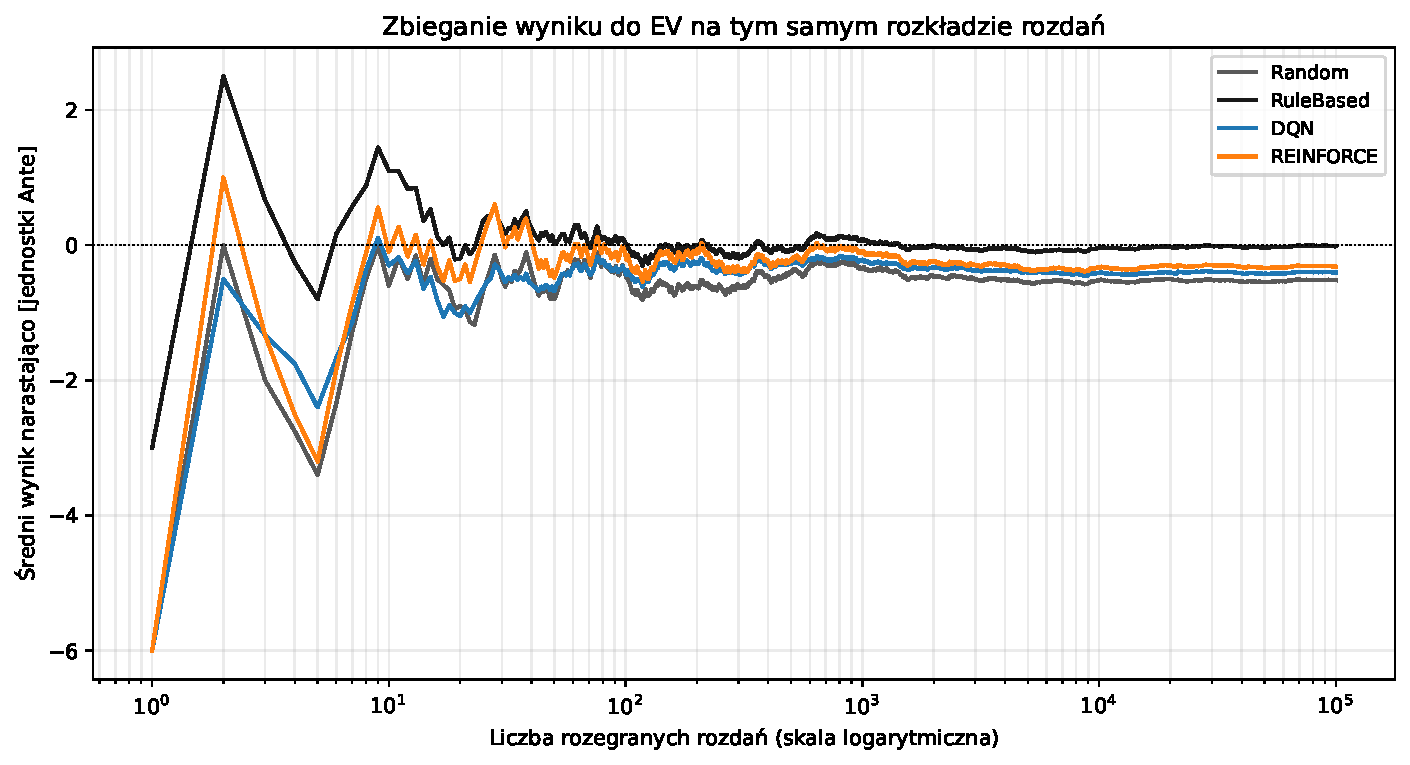
\includegraphics[
        width=0.9\textwidth
    ]{../experiments/results/final_analysis/13_bankroll_curve.pdf}
    \caption{Zbieganie średniego wyniku do EV na współdzielonym
    harmonogramie rozdań.}
    \label{fig:bankroll-curve}
\end{figure}
